\chapter{Les profils UML}
%OMG Unified Modeling LanguageTM (OMG UML),Superstructure
\label{chap.profils-UML}

Un projet de développement de jeu vidéo est un projet de grande envergure. C'est non seulement un projet informatique, mais également un projet de design, un projet artistique visuel et sonore et un projet de scénario.

Un projet de développement de jeu vidéo est très complexe et c'est pour cela que les phases d'analyse et de conception sont essentielles à sa réussite. Il faut analyser les besoins et le domaine et organiser les étapes d'analyse et de conception. Toutes ces données doivent être accessibles et modifiables afin de pouvoir les consulter et les faire évoluer tout au long du projet.

Un outil permettant de modéliser les besoins, les données et la conception d'un logiciel existe déjà : \glsfirst{uml}. UML permet d'effectuer toutes ces actions, mais permet également d'être adapté à un domaine d'application particulier à travers les profils UML. C'est ce que nous allons présenter dans le chapitre présent.


\section{Le langage de modélisation UML}

Le \glsfirst{uml} est un langage de modélisation standardisé permettant de créer des mod\`eles, typiquement sous forme de diagrammes.
Ces diagrammes permettent de visualiser, spécifier, construire et documenter des logiciels, des systèmes et des processus d'affaire.
UML utilise diverses notations,  surtout graphiques, pour exprimer l'architecture, le design ainsi que la mise en \oe{}uvre de logiciels.
Les spécifications du standard UML sont en ligne sur le site de l'OMG (\emph{Object Management Group})~\cite{OMG_UML}.

\gt{Comme indiqu\'e pr\'ec\'emment, sauf certaines exceptions, on
n'utilise pas trop le positionnement [H], i.e., on laisse flotter, on
laisse \LaTeX\ d\'ecider o\`u mettre la figure. Par contre, on met les
figures ou tableaux *avant* la r\'ef\'erence.}


\gt{Dans la figure 4.1: Tu indiques <<Diagrammes structurels>> mais
dans le texte tu parles de <<Diagrammes de structure>>.  Et ce serait
mieux de mettre au singulier aussi, car les autres boites sont au
singulier. Et <<de \underline{de} structures composites>>!}

\gt{Figure 4.2: Idem: parfois Diagrammes, parfois Diagramme. Mettre
singulier partout.}
 
\begin{figure}
    \centering
    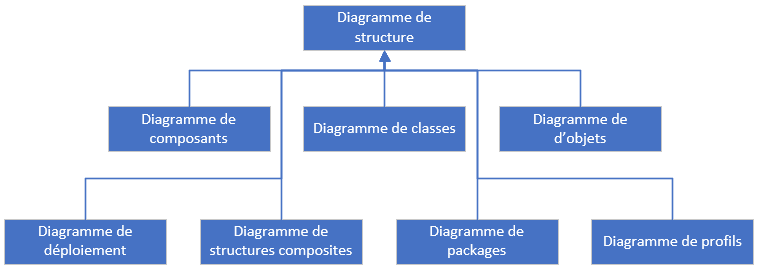
\includegraphics[width=12cm]{10_img/chap4/structure.PNG}
    \caption{Les principaux types de diagrammes de structure d'UML~\cite{OMG_UML}.}
    \label{fig.uml_struc}
\end{figure}

\begin{figure}
    \centering
    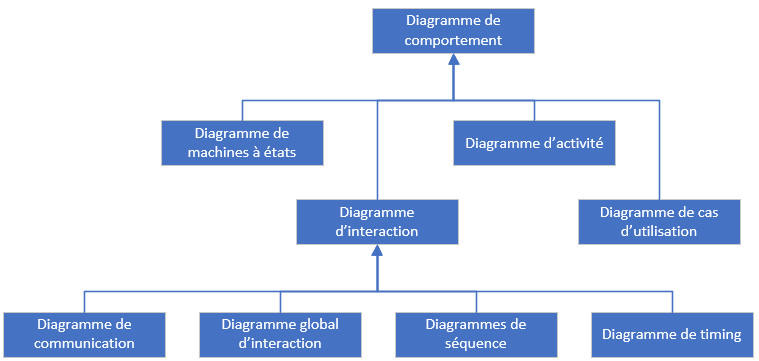
\includegraphics[width=12cm]{10_img/chap4/comportement.PNG}
    \caption{Les principaux types de diagrammes de comportement d'UML~\cite{OMG_UML}.}
    \label{fig.uml_comp}
\end{figure}


\gt{Il vaut mieux utiliser une forme <<active>> --- <<La figure
pr\'esente>> --- qu'une forme passive --- <<Dans la figure sont
pr\'esent\'es\ldots>>.}

La figure~\ref{fig.uml_struc} présente les principaux types de diagrammes de structure proposés par UML,
alors que la figure~\ref{fig.uml_comp} présente les principaux types de diagrammes de comportement.

UML \'etant un langage de modélisation largement connu et bien documenté dans le domaine du g\'enie logiciel,
nous nous concentrons dans le pr\'esent chapitre plus particulièrement à définir les notions nécessaires à la compréhension des mécanismes et des éléments composant les profils UML.



\section{La notion de profil en UML}

\gt{UML pr\'esente diverses notions, qui peuvent \^etre
repr\'esent\'ees de fa\c{c}on graphique ou textuelle.  Donc, en soit,
aucun item UML n'est un diagramme.  Le diagramme est une des
repr\'esentations possibles d'une notion.}


Un profil UML est un m\'ecanisme d'extension, qui
permet d'étendre les éléments d'UML afin d'adapter les mod\`eles et leur contenu à un domaine particulier (par ex.,  domaines d'activité spécifique) ou \`a une plateforme particulière (par ex.,  .NET, J2EE).

Les extensions qu'un profil d\'efinit permettent d'ajouter des caractéristiques aux éléments standards d'UML.
Ces extensions ne peuvent pas \emph{retirer} des caractéristiques, et ce pour ne pas aller à l'encontre de la sémantique standard d'UML.
Un profil se compose  de stéréotypes, de valeurs \'etiquet\'ees (\emph{tagged values}) et de contraintes qui s'appliquent aux éléments de modèles UML tels que les classes, les attributs, les opérations et les activités.

\gt{Pour l'exemple, pas une bonne idée d'avoir une sous-section
numérotée --- parce qu'alors, il y a une seule sous-section numérotée,
ce qui n'est pas d'un bon style.}

\subsection*{Exemple}
%
Afin de mieux comprendre les éléments qui composent un profil, nous allons mettre en place un exemple au fur et à mesure de ce chapitre, en y intégrant divers éléments un \`a la fois.

\begin{figure}
    \centering
    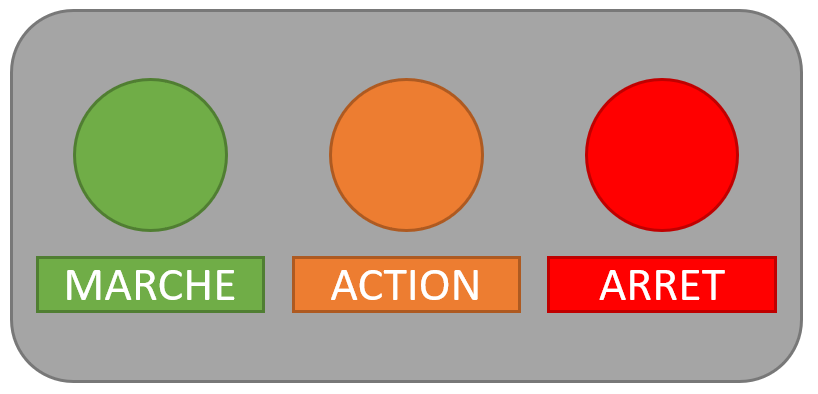
\includegraphics[width=8cm]{10_img/chap4/example.PNG}
    \caption{Le tableau de bord de la machine pour notre exemple de profil UML.}
    \label{fig.uml_ex}
\end{figure}

Prenons un exemple d'un mod\`ele devant représenter un tableau de bord d'une machine composée de trois boutons : \texttt{Marche}, \texttt{Action}, \texttt{Arrêt}.
Chaque bouton a un état <<\texttt{actif}>> ou <<\texttt{inactif}>>, et
chacun a une action qui lui est propre sur la machine contr\^ol\'ee par ces boutons : \texttt{Marche} = démarre la machine; \texttt{Action} = effectue l'action de la machine; \texttt{Arrêt} = termine l'ex\'ecution de la machine.
%
La figure~\ref{fig.uml_ex} illustre un tableau de bord possible pour une telle machine.

%\newpage \GT{A EVITER, sauf a la toute fin, quand on veut fignoler la mise en page!}

\section{Les stéréotypes}
\label{sect.uml.ster}
Les stéréotypes permettent de spécifier des extensions aux métaclasses UML.
Ceci permet d'ajouter des termes spécifiques de vocabulaire à un mod\`ele.
Un stéréotype peut être défini pour divers types d'éléments d'un mod\`ele UML, par exemple, classes, associations, attributs, etc.


\subsection*{Exemple}
%
\begin{figure}
    \begin{center}
    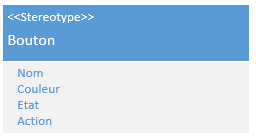
\includegraphics[width=6cm]{10_img/chap4/button.PNG}
    \caption{Un st\'er\'eotype <<\texttt{Bouton}>> permettant de sp\'ecifier les points communs aux diff\'erents boutons.}
    \label{fig.uml_but_definition}
    \end{center}
\end{figure}

Dans la figure~\ref{fig.uml_but_definition}, on remarque la présence d'une flèche noire à tête pleine entre les éléments "\texttt{<<stereotype>> Bouton}" et "\texttt{<<metaclass>>~Class}".
C'est la notation (graphique) UML indiquant que le st\'er\'eotype \texttt{Bouton} \textbf{étend} (\emph{extension}) la métaclasse UML \texttt{Class}.
%
En d'autres mots, le stéréotype \texttt{Bouton} pourra être utilisé pour \emph{annoter des classes.}
%
Signalons aussi qu'une extension, comme on le verra dans le prochain chapitre, peut aussi être utilisée en lien avec la métaclasse \texttt{Association}, ce qui permet alors de stéréotyper une association.

\begin{comment}
\GT{Pas nécessaire... et pas certain pour la multiplicité!?}

La notation d'extension peut inclure différents éléments, mais qui ne sont pas requis dans notre cas comme :
\begin{itemize}
    \item la notation \emph{<<~required~>>} qui indiquerait que l'extension est obligatoire sur chaque élément de \texttt{<<~metaclass~>>Class}.
    \item des multiplicités qui définissent si un objet \texttt{<<~metaclass~>>Class} peut être étendu par un ou plusieurs stéréotypes.
\end{itemize}
\end{comment}

\gt{Dans la figure \ref{fig.uml_but_definition}, tu dois \^etre plus explicite
quant au fait que cela \'etend une classe.
%
Donc, ta boite/classe Bouton doit \^etre une sous-classe d'une boite contenant "<<metaclass>> Class".
%
Voir d\'ebut de la page \url{https://www.uml-diagrams.org/stereotype.html}.}

\gt{Tu devrais utiliser ce stereotype pour d\'efinir au moins un des
boutons, par ex.: "<<bouton>> Marche". Cf. partie <<Stereotype
Application>> de
\url{https://www.uml-diagrams.org/stereotype.html}. Pr\'ef\'erablement
dans une autre figure, possiblement dans la section Tagged values.
Parce que l\`a, tu introduis le stereotype Bouton, mais ensuite tu
utilise celui de Machine, qui n'est pas d\'efini!}


Dans notre exemple, nous avons plusieurs éléments : un tableau de bord, des boutons, des actions que les boutons effectuent.
Un stéréotype, comme celui présenté à la Figure~\ref{fig.uml_but_definition}, pourrait être d\'efini afin de sp\'ecifier les caractéristiques communes des boutons.




Une fois d\'efini, ce st\'er\'eotype pourra alors \^etre utilis\'e pour
d\'efinir diff\'erentes instances de \texttt{Bouton}, tel qu'illustré à la Figure~\ref{fig.uml_marche}.


%\newpage

\section{Les valeurs \'etiquet\'ees}

Les valeurs \'etiquet\'ees (\emph{tagged values}) permettent d'ajouter \`a un \'el\'ement des propriétés qui lui sont spécifiques.
Plus pr\'ecis\'ement, ce m\'ecanisme permet d'ajouter de l'information spécifique aux éléments \`a l'aide de paires clé/valeur.
%Les attributs présents dans un stéréotype seront affichés visuellement dans une classe faisant usage du stéréotype.
Ces couples clé/valeur sont indiqués comme illustré dans la Figure~\ref{fig.uml_marche}.

\gt{Je ne comprends pas la derni\`ere phrase!?}

\subsection*{Exemple}
%
\eh{J'ai placé un [H] sur cette figure car elle passe dans la subsection précédente. cela pose un probleme de compréhension}
\begin{figure}[H]
    \begin{center}
    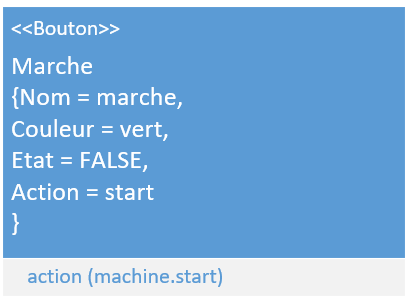
\includegraphics[width=7cm]{10_img/chap4/start.PNG}
    \caption{Une classe pour \texttt{Marche}, spécifiée à l'aide du stéréotype \texttt{Bouton} et des valeurs \'etiquet\'ees.}
    \label{fig.uml_marche}
    \end{center}
\end{figure}

\gt{Dans la figure 4.5: les noms des stéréotypes et classes débutent par une majuscule, mais pas les attributs, qui doivent débuter par une minuscule: nom, couleur, etat, action.}

\gt{Voir mon courriel: en UML 2.0, il semble que les tagged values
doivent être mises dans une sous-boite, avec le nom du stéréotype.}

\gt{Ci-haut: les explications portent sur l'ancien exemple, pas le
nouveau avec le Bouton, donc à réécrire.}

\gt{Je crois, comme indiqu\'e plus haut, qu'une utilisation de Bouton serait pr\'ef\'erable.}

%\newpage

\section{Les contraintes}
Les contraintes sont des propriétés spécifiques, qui permettent de sp\'ecifier des conditions additionnelles sur un modèle.
Ces conditions peuvent être appliquées à une ou plusieurs classes, à un ou plusieurs attributs, à une ou plusieurs relations entre classes.
Une contrainte est représent\'ee, dans un modèle, sous la forme d'une note indiquant une phrase qui exprimant la contrainte entre crochets ou encore, de fa\c{c}on plus formelle, sous la forme d'une contrainte OCL~\cite{OCL}.

\subsection*{Exemple}
%
\eh{J'ai placé un [H] sur cette figure car elle passe dans la subsection précédente. cela pose un probleme de compréhension}
\begin{figure}[H]
    \begin{center}
    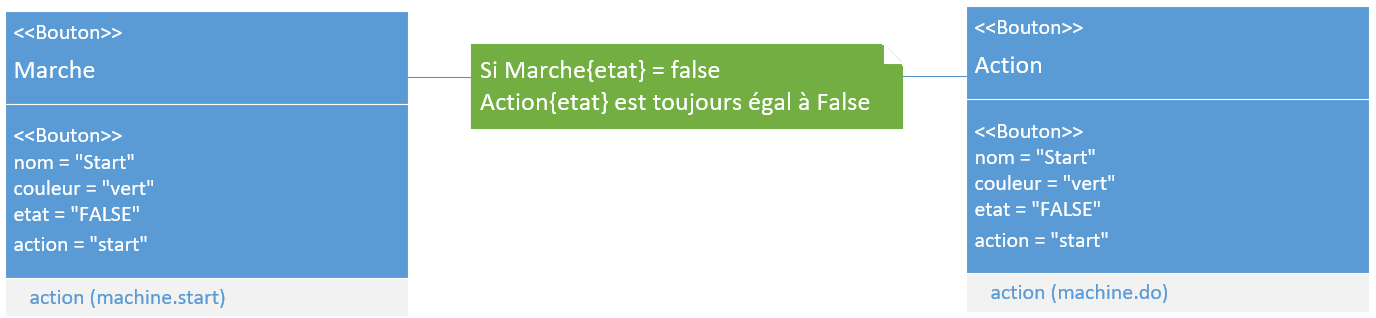
\includegraphics[width=\linewidth]{10_img/chap4/constraint.PNG}
    \caption{Des contraintes sp\'ecifiant des conditions sur des \'el\'ements d'un modèle.}
    \label{fig.uml_con}
    \end{center}
\end{figure}

\gt{Dans la figure: Etat => etat (attribut, minuscule), Nom => nom,
etc. Et j'écrirais plutôt <<Si Marche(etat) = false Alors Action(etat)
= false>>}

Nous trouvons l'exemple d'une contrainte dans la Figure~\ref{fig.uml_con}, entre les boutons \texttt{Marche} et \texttt{Action}.
Cette contrainte énonce que si l'état du bouton \texttt{Marche} est \texttt{false}, alors l'état du bouton \texttt{Action} sera lui aussi \texttt{false},
ce qui signifie que l'action de la machine ne peut pas être effectuée si la machine est à l'arrêt.
On pourra alors sp\'ecifier, dans un diagramme UML, la contrainte présent\'ee dans la figure~\ref{fig.uml_con}.

%\newpage

\section{Les ic\^ones}
Lorsque la taille d'un modèle devient importante, il peut devenir difficile de s'y retrouver parmi les nombreux st\'er\'eotypes.
Dans ce cas, l'association d'ic\^ones aux st\'er\'eotypes peut être une solution int\'eressante à mettre en place dans le cas d'un profil dans un domaine d'activité spécifique.
Une représentation graphique simple --- une ic\^one --- peut ainsi être attribuée à un type d'élément spécifique du modèle.

\subsection*{Exemple}
%
\eh{J'ai placé un [H] sur cette figure car elle passe dans la subsection précédente. cela pose un probleme de compréhension}
\begin{figure}[H]
    \begin{center}
    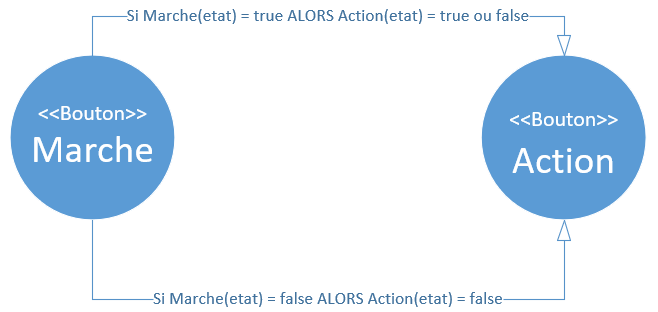
\includegraphics[width=12cm]{10_img/chap4/etat.PNG}
    \caption{Une ic\^one spécifique associ\'ee aux boutons.}
    \label{fig.uml_img}
    \end{center}
\end{figure}

Dans notre exemple, une machine est composée de trois boutons.
On peut alors choisir, par exemple, d'attribuer une ic\^one spécifique aux boutons afin de les différencier des autres éléments, tel qu'illustr\'e dans la figure~\ref{fig.uml_img}.



%\newpage

\section{L'utilisation d'un profil UML pour la conception de jeux vidéos}


UML est un langage de modélisation permettant de représenter divers types de systèmes et permettant de les documenter de manière rigoureuse en apportant les caractéristiques suivantes :

\begin{itemize}
    \item UML est un langage formel et normalisé;
    \item UML est manipulable avec de nombreux outils déjà approuvés;
    \item UML est un support de communication performant;
    \item UML est un langage qui permet le contrôle des versions et la conservation de l'information de manière efficace.
\end{itemize}

\gt{Ci-haut: Pas certain que j'aime la comparaison avec les mind maps.
Dans mon esprit, un mind map a un r\^ole tout \`a fait diff\'erent ---
plus exploratoire, parce que plus libre, avec moins de
contraintes. Donc, je crois que tes items pourraient rester, mais sans
insister sp\'ecifiquement que c'est par rapport aux mind maps.}



Cependant, UML est un langage de modélisation tellement étendu qu'il permet de <<tout faire>> --- ou presque ---, ce qui rend le langage difficile à appréhender.
De plus, UML est prévu à l'origine pour représenter des systèmes logiciels quelconques, donc avec un vocabulaire générique.


Dans les chapitres précédents, nous avons établi une liste de points importants concernant la conception de jeux vidéos.
Nous pensons qu'un profil UML serait un outil int\'eressant pour répondre aux besoins de modélisation d'un GDD.
La mise en place d'un profil UML aurait plusieurs avantages :
\begin{itemize}
    \item En utilisant un profil, il est possible de simplifier la compréhension des différents éléments UML utilisés pour exprimer un concept, ce qui permet de réduire la quantité de connaissances à acquérir pour se servir d'UML dans le cadre de la rédaction d'un GDD.

    \item Les stéréotypes permettent d'intégrer des notions spécifiques au \emph{game design}.

    \item Les valeurs \'etiquet\'ees permettent d'ajouter des propriétés spécifiques aux nouveaux éléments introduits par les st\'er\'eotypes.

    \item Des contraintes peuvent être sp\'ecifi\'ees dans un profil afin d'éviter des erreurs.

    \item Des ic\^ones peuvent être associ\'ees aux éléments du modèle pour faciliter sa compréhension.

    \item Les outils supportant UML sont nombreux et efficaces. Ils sont déjà présents sur le marché et répondent aux besoins de la modélisation UML.
\end{itemize}


\gt{Ci-haut: 2e item: je ne comprends l'histoire de <<port\'ee>> des objets!?}

Grâce aux ajustements et extensions permis par les profils, UML semble être un langage int\'eressant pour permettre la représentation graphique d'un GDD.
C'est pourquoi, dans le prochain chapitre, nous proposons un profil UML permettant la description des éléments d'un GDD.
